%!TEX root = paper.tex

\section{Browsers}
\label{sec:browsers}

Modern web browsers do not just load static pages, but can also handle pages that have similar
complexity to native applications.
From application suites such as the Google Apps\footnote{\url{https://apps.google.com}} to games
based on the Unreal Engine\footnote{\url{https://blog.mozilla.org/blog/2015/02/24/unreal-engine-4-7-binary-release-includes-html5-export-3/}},
modern browsers have the ability to handle much more than simple static pages.
\figref{fig:browser} shows the steps in processing a site.
While the naming is specific to the Servo browser, similar steps are used in all modern browsers.\footnote{\url{www.html5rocks.com/en/tutorials/internals/howbrowserswork/}}
\begin{figure*}%[ht]
  \begin{center}
    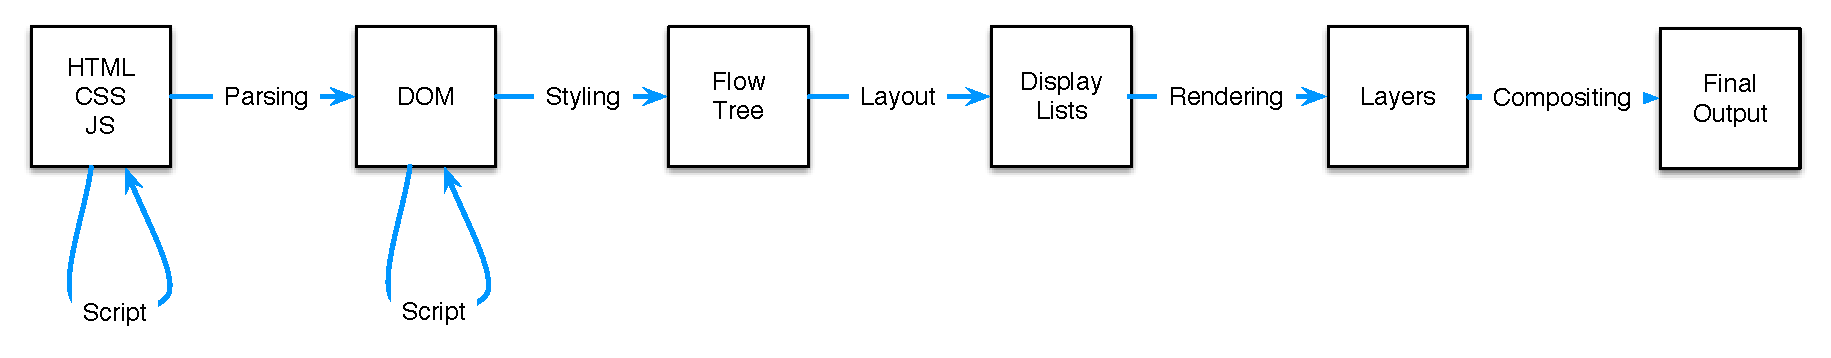
\includegraphics[scale=0.7]{pics/browser}
  \end{center}%
  \caption{Processing stages and intermediate representations in a browser engine.}
  \label{fig:browser}
\end{figure*}%

\subsection{Parsing HTML and CSS}

A URL identifies a resource to load.
This resource usually consists of HTML, which is then parsed and typically turned into a Document Object
Model (DOM) tree.
From a programming languages standpoint, there are several interesting aspects of the parser design
for HTML.
First, though the specification allows the browser to abort on a parse error\footnote{\url{https://html.spec.whatwg.org/multipage/syntax.html#parsing}},
in practice browsers follow the recovery algorithms described in that specification and make a best attempt to
load any page given to them.
Second, due to the presence of the \lstinline[language=HTML]{<script>} tag, the token stream can be modified
during operation.
For example, the below example that injects a close tag for the script block works in all modern browsers.
\begin{lstlisting}[language=HTML]
  <html>
    <script>
      document.write (``</script>
    <li>this shows up just fine, thanks</li>
  </html>
\end{lstlisting}
Finally, since resource loading is such a large factor in the latency of loading many webpages (particularly on mobile),
all modern parsers also perform token stream scanning and prefectch of resources likely to be required. CITE

\subsection{Layout}

After constructing the DOM and determining the set of styles defined in the Cascading Style Sheets (CSS) that has
been loaded, those styles are applied to the DOM and a new tree that represents the elements for display is
created.
This process can create many more elements than previously existed in the DOM --- for example, when a list item is
styled to have an associated counter glyph.

\subsection{Painting}

Once all of the elements to appear on screen have been computed, these elements are painted into memory buffers or
directly to graphics surfaces.
The order of painting these elements is well-defined by the standard\footnote{\url{http://www.w3.org/TR/CSS21/zindex.html#painting-order}}.

\subsection{Scripting}

Whether through timers, \lstinline[language=HTML]{<script>} blocks in the HTML, user interactions, or other event handlers,
JavaScript (JS) code may execute at any point during parsing, layout, and painting or afterwards during display.
These scripts can modify the DOM tree, which may require rerunning the layout and painting passes in order to update
the output.
Most modern browsers use some form of dirty bit marking to attempt to minimize the recalculations during this process.


%%% Local Variables: 
%%% mode: latex
%%% TeX-master: "paper"
%%% End: 
